%==========================================================================%
% MAIN PREAMBLE 
%==========================================================================%
\documentclass[12pt,letterpaper]{report} % Single-sided printing for the library
% \documentclass[12pt,twoside]{report} % Double-sided printing
\usepackage[intlimits]{amsmath}
\usepackage[utf8]{inputenc}
\usepackage{amsfonts,amssymb}
\DeclareSymbolFontAlphabet{\mathbb}{AMSb}
% \usepackage{natbib}
% \usepackage{apalike}
\usepackage{float}
\usepackage[]{caption,subcaption}
\setcaptionmargin{0.5in}
\usepackage{fancyhdr}
%\usepackage{fancyheadings} % what does this do?
\usepackage{fancybox}
\usepackage{ifthen}
\usepackage{template_style} % style package and also some layout stuff
\usepackage{lscape,afterpage}
\usepackage{xspace}
% \usepackage{epstopdf} % what does this do?

\usepackage{appendix}

% https://tex.stackexchange.com/questions/13509/biblatex-in-a-nutshell-for-beginners
% if I get the error, ".bbl not created by bib latex", run biber $, where $ is the basename of the main .tex file, then rerun the build
\usepackage{biblatex}
\addbibresource{thesis.bib}
% \addbibresource(othersfiles.bib) % if I ever split up the bibiliography add multiple resources like this

%feynman digram package

% \usepackage{tikz-feynman} % doesn't work out of the gate, wants LuaLaTex - see https://jpellis.me/projects/tikz-feynman/
% \tikzfeynmanset{compat=1.1.0} 
\usepackage{tikz-feynhand} % simpler version of tikz-feynman - see https://ctan.org/pkg/tikz-feynhand?lang=en


%==========================================================================%
%%% graphicx and pdf creation
\usepackage{graphicx}

\usepackage{hyperref} % set up this package last (or almost last anyways)
\hypersetup{
    colorlinks=true,
    linkcolor=red,
    urlcolor=blue,
    citecolor=blue
}

% \usepackage{glossaries} % might be able to use this to make an alphabetically ordered list of abbreviations - needs to be set up after hyperref

%==========================================================================%
% customized commands can be placed here
%\newcommand{\figref}[1]{Figure~\ref{#1}}
%\newcommand{\chapref}[1]{Chapter~\ref{#1}}
%\newcommand{\latex}{\LaTeX\xspace}
%==========================================================================%

%==========================================================================%
% BEGIN
%==========================================================================%
\begin{document}

% The preliminary pages
\include{Preliminary/OpeningPages} % putting .text at the end is something different from leaving it off here
\cleardoublepage

%%%%%%%%%%%%%%%%%%%%%%%%%%%%%%%%%%%%%%%%%

% The content of the thesis
%!TEX root = ../thesis.tex

\thispagestyle{myheadings}
\graphicspath{{Body/Figures/Theory/}}

\chapter{Introduction}
\label{chapter:Introduction}

The prevailing theory for particle physics, the Standard Model (SM), has had tremendous success in describing our universe. It has been used to predict and explain a wide variety of phenomena and particles, their properties and interactions, to great precision. However, in spite of its success in explaining nearly all experimental results, there exist unanswered questions about our universe. Some of these include the matter-antimatter asymmetry, the source of mass for the neutrinos, the existence of dark matter, and an inability to fully incorporate our best theory of gravitation. Many particle physics experiments are being devised and conducted around the world in order to shed light on these questions and improve our understanding of reality. One such particular experiment is the Fermilab Muon \gmtwo Experiment (E989) underway at the Fermi National Accelerator Laboratory (FNAL) located in Batavia, Illinois.

I have been a part of the E989 experiment since I began my graduate degree six years ago. Three years ago I moved from Boston to Batavia to be where the action is. This dissertation will describe in detail the work which I have done for the experiment. Chapter 1 will provide experimental and theoretical background to the experiment, as well its motivation. Chapter 2 will  describe the experimental principle. Chapter 3 will describe the magnetic field portion of the experiment, and magnetic field simulations I conducted. Chapter 4 will describe the straw tracking detectors and their measurements, including the track fitting I wrote. Chapter 5 will describe the frequency measurement portion of the experiment, and detail the analysis results from data taken in the first half of 2018. Finally, Chapter 6 will concluded the thesis and the important results contained within.


\section{Magnetic Dipole Moments}
\label{sec:MDMs}

In order to understand the purpose of the Fermilab Muon \gmtwo Experiment, first we need to understand what the $g$ in \gmtwo is, which is what the experiment is measuring. All particles have intrinsic properties which describe those particles. One of those properties is the so called magnetic dipole moment. This property of a particle is related to its spin through the equation
		\begin{align}
            \vec{\mu} = g \frac{Qe}{2m} \vec{s},
        \label{eq:magneticmoment}
		\end{align}
where $\vec{\mu}$ is the magnetic dipole moment of a particle, $\vec{s}$ is its spin vector, $m$ is its mass, $e$ is the elementary charge, $Q = \pm1$, and \g is the so called "g-factor". (Here and following $c$ and $\hbar$ have been set to 1.) \g is some measureable and predictable constant, which as shown in \equref{eq:magneticmoment} simply relates the magnetic moment of a particle to its spin angular momentum. 

In a Dirac theory, \g is equal to 2 for spin-1/2 particles with no internal structure \cite{Dirac}. See Appendix~\ref{gDirac} for a derivation of this result. It turns out however, that \g is not quite equal to 2 even for these types of simple particles. Motivated by early experimental discrepencies such as the measurements of the hyperfine structure in hydrogen \cite{EarlyHyperfine1}, in 1948 Schwinger calculated the first "radiative correction" to the electron magnetic moment \cite{Schwinger}. In a quantum field theory, interactions of the particle with virtual particles in loops will contribute to the value of \g. In this context it is nicer to recast the magnetic moment formula as 
		\begin{equation}
		\begin{aligned}
            \vec{\mu} &= 2(1+a) \frac{Qe}{2m} \vec{s}, \\
            a &= \frac{g-2}{2},
        \label{eq:anamoly}
		\end{aligned}
		\end{equation}
where $a$ is called the "anamolous" part of the magnetic moment, and contains all higher order corrections. The first correction calculated to $a$ by Schwinger was $a = \alpha/2\pi \approx 0.00116$, where $\alpha$ is the fine structure constant. By measuring $a$, the SM theory (and extensions to it) can be tested. The measurement of the anamolous piece of the muon is indeed where the Fermilab Muon \gmtwo Experiment gets its name.


\subsection{Why the muon and not the electron?}

The magnetic moment of the electron has been measured extraordinarily precisely, to .28 parts per trillion (ppt) \cite{ElectronMDM}. It has been used to test SM theory extensively, and specifically the QED portion of it. Because the electron is so light, the contributions to $a_{e}$ come almost exclusively from QED. This is because the various contributions from both the weak and hadronic sectors contain couplings which depend on the mass of the particle squared. It is for this reason that the magnetic moment of the muon is such an interesting quantity to measure. Since the muon is approximately 200 times heavier than the electron, the senstivity of \amu to radiative corrections is approximately 4000 times greater than that for the the electron.


\section{Standard Model Contributions to \amu}
\label{sec:Theory}


Before experimental results have any real meaning, they need a theory with which to compare. The latest theoretical predictions for the muon magnetic moment will be presented here. The contributions to \amu can be summed from separate pieces relating to different parts of the SM. These include the quantum-electrodynamics (QED) corrections purely from other leptons and photons, the electroweak (EW) corrections from interactions with the weak force bosons $W^{\pm}$ and $Z^{0}$, and the hadronic corrections from interactions with hadrons: 
		\begin{align}
            a_{\mu}^{\text{SM}} = a_{\mu}^{\text{QED}} + a_{\mu}^{\text{EW}} + a_{\mu}^{\text{Had}}
		\end{align}
The QED corrections are very well understood and have been calculated to very high order. The electroweak corrections are harder to calculate, but due to the heavy masses of the force carrying bosons and by extension weaker couplings, are only required to be known up to two loop level. And indeed they are. Finally, the hadronic contributions are where most of the theoretical uncertainties lie, and where most active work is going on. Indeed there are also some data-driven approaches to the hadronic contributions which are interesting and will be discussed in a following section.






-just put words down on the page, keep it short and simple, I can go back and add detail where necessary, I'll have to do a lot of editing anyways
-dont worry about the ordering of sections exactly either
-check Saskia's thesis for the latest theoretical results


- see papers cited in my HEP2 class paper - and then look for new ones
- Fred Jegerlehner's book




\subsection{QED}
\label{subsec:QED}

The QED contributions to \amu stem solely from loops with virtual leptons and photons. They have been calculated up to 5 loop levels from over 12,000 Feynman diagrams \cite{Kinoshita1,Kinoshita2}. The first couple of diagrams including the Dirac $g = 2$ and Schwinger diagrams are shown in \figref{fig:QEDDiagrams}. The value is
		\begin{align}
            a_{\mu}^{\text{QED}} = (11658471.8971 \pm 0.007) \times 10^{10}.
		\end{align}
Over 99\% of the value of \amu comes from the QED parts, but the error is much smaller than the other contributions and than the experimental uncertainty.

\begin{figure}[]
\centering
	\begin{subfigure}[t]{0.3\textwidth}
	\centering
		\begin{tikzpicture}[baseline=(o.base)]
		\begin{feynhand}
		\large
		\setlength{\feynhandlinesize}{1pt}
		\vertex [dot] (o) at (0,0);
		\vertex (a) at (-2,-2) {$l$}; 
		\vertex (b) at (2,-2) {$\overline l$}; 
		\vertex (c) at (0,2) {B};
		\propag [fermion] (a) to (o);
		\propag [anti fermion] (b) to (o);
		\propag [photon] (c) to [edge label = $\gamma$] (o);
		\end{feynhand}
		\end{tikzpicture}
	\caption{Dirac result, $g=2$.}
	\end{subfigure}
	\hspace{3mm}
	\begin{subfigure}[t]{0.3\textwidth}
	\centering
		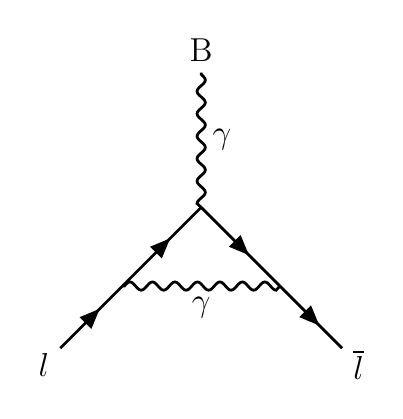
\begin{tikzpicture}[baseline=(o.base)]
		\begin{feynhand}
		\large
		\setlength{\feynhandlinesize}{1pt}
		\vertex [dot] (o) at (0,0);
		\vertex (a) at (-2,-2) {$l$}; 
		\vertex (b) at (2,-2) {$\overline l$}; 
		\vertex (c) at (0,2) {B};
		\vertex (d) at (-1,-1);
		\vertex (e) at (1,-1);
		\propag [fermion] (a) to (d);
		\propag [fermion] (d) to (o);
		\propag [anti fermion] (b) to (e);
		\propag [anti fermion] (e) to (o);
		\propag [photon] (c) to [edge label = $\gamma$] (o);
		\propag [photon] (d) to [edge label' = $\gamma$] (e);
		\end{feynhand}
		\end{tikzpicture}
	\caption{The first loop diagram, calculated by Schwinger.}
	\end{subfigure}
	\hspace{3mm}
	\begin{subfigure}[t]{0.3\textwidth}
	\centering
		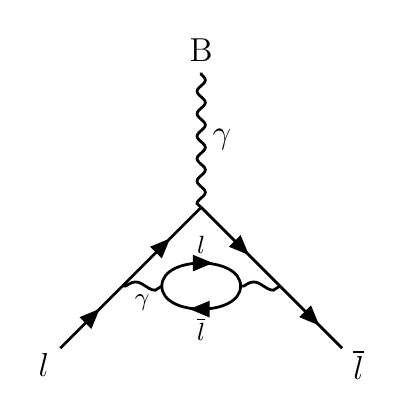
\begin{tikzpicture}[baseline=(o.base)]
		\begin{feynhand}
		\large
		\setlength{\feynhandlinesize}{1pt}
		\vertex [dot] (o) at (0,0);
		\vertex (a) at (-2,-2) {$l$}; 
		\vertex (b) at (2,-2) {$\overline l$}; 
		\vertex (c) at (0,2) {B};
		\vertex (d) at (-1,-1);
		\vertex (e) at (1,-1);
		\vertex (f) at (-.5,-1);
		\vertex (g) at (+.5,-1);
		\propag [fermion] (a) to (d);
		\propag [fermion] (d) to (o);
		\propag [anti fermion] (b) to (e);
		\propag [anti fermion] (e) to (o);
		\propag [photon] (c) to [edge label = $\gamma$] (o);
		\small
		\propag [boson] (d) to [edge label' = $\gamma$] (f);
		\propag [boson] (g) to (e);
		\propag [fermion] (f) to [half left, edge label = $l$] (g);
		\propag [anti fermion] (f) to [half right, edge label' = $\overline l$] (g);
		\end{feynhand}
		\end{tikzpicture}
	\caption{A two loop diagram.}
	\end{subfigure}
\caption[QEDDiagrams]{The first of many QED diagrams contributing to $a$. B is a magnetic field. Feynman diagrams made with \cite{tikz-feynman,tikz-feynhand}.}	
\label{fig:QEDDiagrams}
\end{figure}



\subsection{Electroweak}
\label{subsec:Electroweak}

The electroweak contributions to \amu are known to two loop level, with some 3 loop parts estimated. The contributions stem from couplings with the heavy weak gauge bosons. Because the couplings to these heavy bosons are small, the electroweak contributions to \amu are small. The different one loop diagrams and an example two loop diagram are shown in \figref{fig:EWDiagrams}. The value of the elctroweak contributions is
		\begin{align}
            a_{\mu}^{\text{EW}} = (15.12 \pm 0.1) \times 10^{10}.
		\end{align}
with improvements having been made recently \cite{EW1,EW2}. Again the error on these contibutions are small compared to the hadronic contributions discussed next, as well as the experimental uncertainties.


\begin{figure}[]
\centering
	\begin{subfigure}[t]{0.3\textwidth}
	\centering
		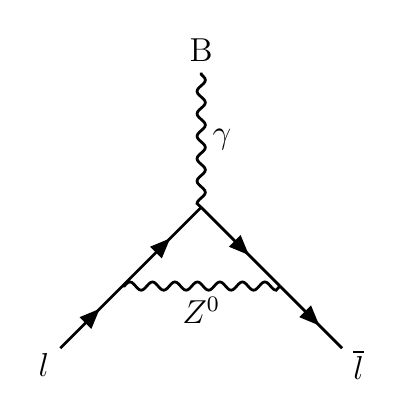
\begin{tikzpicture}[baseline=(o.base)]
		\begin{feynhand}
		\large
		\setlength{\feynhandlinesize}{1pt}
		\vertex [dot] (o) at (0,0);
		\vertex (a) at (-2,-2) {$l$}; 
		\vertex (b) at (2,-2) {$\overline l$}; 
		\vertex (c) at (0,2) {B};
		\vertex (d) at (-1,-1);
		\vertex (e) at (1,-1);
		\propag [fermion] (a) to (d);
		\propag [fermion] (d) to (o);
		\propag [anti fermion] (b) to (e);
		\propag [anti fermion] (e) to (o);
		\propag [photon] (c) to [edge label = $\gamma$] (o);
		\propag [boson] (d) to [edge label' = $Z^{0}$] (e);
		\end{feynhand}
		\end{tikzpicture}
	\caption{Exchange of a virtual $Z^{0}$ boson.}
	\end{subfigure}
	\hspace{3mm}
	\begin{subfigure}[t]{0.3\textwidth}
	\centering
		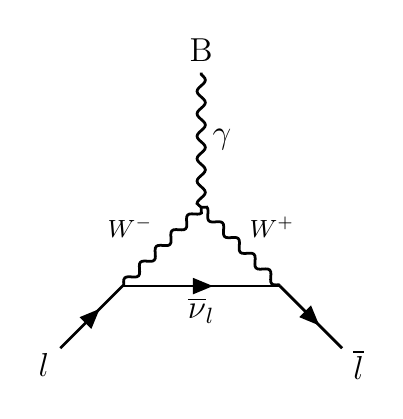
\begin{tikzpicture}[baseline=(o.base)]
		\begin{feynhand}
		\large
		\setlength{\feynhandlinesize}{1pt}
		\vertex [dot] (o) at (0,0);
		\vertex (a) at (-2,-2) {$l$}; 
		\vertex (b) at (2,-2) {$\overline l$}; 
		\vertex (c) at (0,2) {B};
		\vertex (d) at (-1,-1);
		\vertex (e) at (1,-1);
		\propag [fermion] (a) to (d);
		\propag [anti fermion] (b) to (e);
		\propag [photon] (c) to [edge label = $\gamma$] (o);
		\propag [fermion] (d) to [edge label' = $\overline \nu_{l}$] (e);
		\small
		\propag [boson] (d) to [edge label = $W^{-}$] (o);
		\propag [boson] (e) to [edge label' = $W^{+}$] (o);
		\end{feynhand}
		\end{tikzpicture}
	\caption{Weak loop with $W$ bosons.}
	\end{subfigure}
	\hspace{3mm}
	\begin{subfigure}[t]{0.3\textwidth}
	\centering
		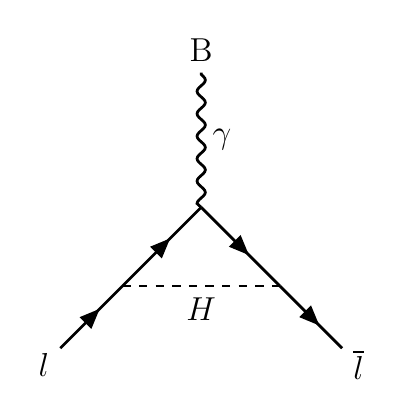
\begin{tikzpicture}[baseline=(o.base)]
		\begin{feynhand}
		\large
		\setlength{\feynhandlinesize}{1pt}
		\vertex [dot] (o) at (0,0);
		\vertex (a) at (-2,-2) {$l$}; 
		\vertex (b) at (2,-2) {$\overline l$}; 
		\vertex (c) at (0,2) {B};
		\vertex (d) at (-1,-1);
		\vertex (e) at (1,-1);
		\propag [fermion] (a) to (d);
		\propag [fermion] (d) to (o);
		\propag [anti fermion] (b) to (e);
		\propag [anti fermion] (e) to (o);
		\propag [photon] (c) to [edge label = $\gamma$] (o);
		\propag [scalar] (d) to [edge label' = $H$] (e);
		\end{feynhand}
		\end{tikzpicture}
	\caption{Exchange of a Higgs boson.}
	\end{subfigure}

	\begin{subfigure}[]{0.4\textwidth}
	\centering
		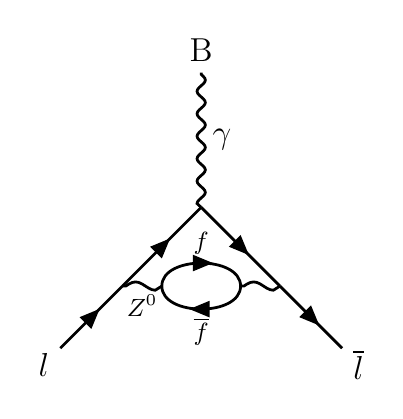
\begin{tikzpicture}[baseline=(o.base)]
		\begin{feynhand}
		\large
		\setlength{\feynhandlinesize}{1pt}
		\vertex [dot] (o) at (0,0);
		\vertex (a) at (-2,-2) {$l$}; 
		\vertex (b) at (2,-2) {$\overline l$}; 
		\vertex (c) at (0,2) {B};
		\vertex (d) at (-1,-1);
		\vertex (e) at (1,-1);
		\vertex (f) at (-.5,-1);
		\vertex (g) at (+.5,-1);
		\propag [fermion] (a) to (d);
		\propag [fermion] (d) to (o);
		\propag [anti fermion] (b) to (e);
		\propag [anti fermion] (e) to (o);
		\propag [photon] (c) to [edge label = $\gamma$] (o);
		\small
		\propag [boson] (d) to [edge label' = $Z^{0}$] (f);
		\propag [boson] (g) to (e);
		\propag [fermion] (f) to [half left, edge label = $f$] (g);
		\propag [anti fermion] (f) to [half right, edge label' = $\overline f$] (g);
		\end{feynhand}
		\end{tikzpicture}
	\caption{Second order weak diagram.}
	\end{subfigure}
\caption[EWDiagrams]{First order (and one second) weak diagrams contributing to $a$. B is a magnetic field. Feynman diagrams made with \cite{tikz-feynman,tikz-feynhand}.}	
\label{fig:EWDiagrams}
\end{figure}


\subsection{Hadronic}
\label{subsec:Hadronic}

The hadronic contributions to \amu stem from interactions with hadrons. Because they cannot be calculated perturbatively at low energies due to the QCD nature of these particles, these calculations comprise the dominant uncertainty in the SM calculation, and make their error estimation extra important when comparing to experiment. These contributions can be separated into two parts. 


\subsection*{Hadronic Vacuum Polarization}
\label{subsec:HVP}

The first of these hadronic contribution parts is the hadronic vacuum polarization part (HVP), the first order diagram of which is shown in \figref{fig:HVP1}. There are two main prescriptions for calculating these contributions. The first is to relate the virtual hadron production within these loops to real hadron production through dispersion theory \cite{Jeger}. The leading order contribution can be written as 
		\begin{align}
            a_{\mu}^{\text{HVP;LO}} = \Big(\frac{\alpha m_{\mu}}{3\pi}\Big)^{2} \int_{m_{\pi}^{2}}^{\infty} \frac{ds}{s^{2}} K(s) R(s)
		\end{align}
where $K(s)$ is some kinematic factor, and $R(s)$ is a ratio of cross-sections
		\begin{align}
            R(s) = \frac{\sigma(e^{+}e^{-} \rightarrow \text{hadrons})}{\sigma(e^{+}e^{-} \rightarrow \mu^{+}\mu^{-})}.
		\end{align}
The cross-section data for this relation has been measured in parts by various experiments, including KLOE, BaBar, and BESIII \cite{KLOE,BaBar,BESIII}. (Name other experiments? (Belle, VEPP-2000) would then need to cite them somehow.) The analysis by \refref{Keshavarzi:2018mgv} gives results as 
		\begin{equation}
		\begin{aligned}
            a_{\mu}^{\text{HVP;LO}} &= (693.26 \pm 2.46) \times 10^{10}, \\
            a_{\mu}^{\text{HVP;NLO}} &= (-9.82 \pm 0.04) \times 10^{10}, 
		\end{aligned}
		\end{equation}
where $a_{\mu}^{\text{HVP;NLO}}$ is the next to leading order calculation. This calculation is consistent with \refref{HVP2}.

-should I mention the optical theorem?

\begin{figure}[]
\centering
	\begin{subfigure}[t]{0.4\textwidth}
	\centering
		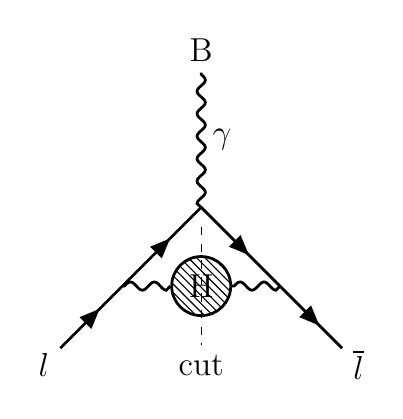
\begin{tikzpicture}[baseline=(o.base)]
		\begin{feynhand}
		\large
		\setlength{\feynhandlinesize}{1pt}
		\vertex [dot] (o) at (0,0);
		\vertex (a) at (-2,-2) {$l$}; 
		\vertex (b) at (2,-2) {$\overline l$}; 
		\vertex (c) at (0,2) {B};
		\vertex (d) at (-1,-1);
		\vertex (e) at (1,-1);
		\vertex [NWblob] (f) at (0,-1) {H};
		\propag [fermion] (a) to (d);
		\propag [fermion] (d) to (o);
		\propag [anti fermion] (b) to (e);
		\propag [anti fermion] (e) to (o);
		\propag [photon] (c) to [edge label = $\gamma$] (o);
		\propag [photon] (d) to (f);
		\propag [photon] (f) to (e);
		\draw [dashed] (0,-.25) to (0,-1.75);
		\node at (0, -2) {cut};
		\end{feynhand}
		\end{tikzpicture}
	\caption{The first order HVP diagram. The blob H in the middle indicates any combination of hadrons which satisfy the Feynman rules. By making a 'cut' at the virtual hadrons part, this diagram can be related to the one on the right.} 
	\label{fig:HVP1}
	\end{subfigure}
	\hspace{3mm}
	\begin{subfigure}[t]{0.4\textwidth}
	\centering
		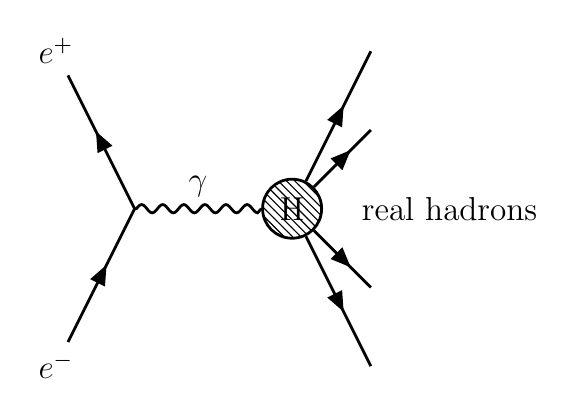
\begin{tikzpicture}[baseline=(o.base)]
		\begin{feynhand}
		\large
		\setlength{\feynhandlinesize}{1pt}
		\vertex [dot] (o) at (-1,0);
		\vertex (a) at (-2,-2) {$e^{-}$}; 
		\vertex (b) at (-2,2) {$e^{+}$}; 
		\vertex [NWblob] (c) at (1,0) {H};
		\vertex (d) at (2,2); 
		\vertex (e) at (2,1); 
		\vertex (f) at (2,-1); 
		\vertex (g) at (2,-2); 
		\propag [fermion] (a) to (o);
		\propag [anti fermion] (b) to (o);
		\propag [photon] (o) to [edge label = $\gamma$] (c);
		\propag [fermion] (c) to (d);
		\propag [fermion] (c) to (e);
		\propag [fermion] (c) to (f);
		\propag [fermion] (c) to (g);
		\node at (3, 0) {real hadrons};
		\end{feynhand}
		\end{tikzpicture}
	\caption{The Feynman diagram for electron positron annihilation to hadrons. This can be related to the diagram on the left.}
	\label{fig:HVP2}
	\end{subfigure}
\caption[HVP]{Feynman diagrams made with \cite{tikz-feynman,tikz-feynhand}.}	
\label{fig:HVP}
\end{figure}



The second prescription is to .... lattice ... 



\subsection*{Hadronic Light-by-Light}
\label{subsec:HLbL}

The second of these hadronic contributions parts is a higher order 4 photon blahblah


\begin{figure}[]
\centering
	\begin{subfigure}[t]{0.4\textwidth}
	\centering
		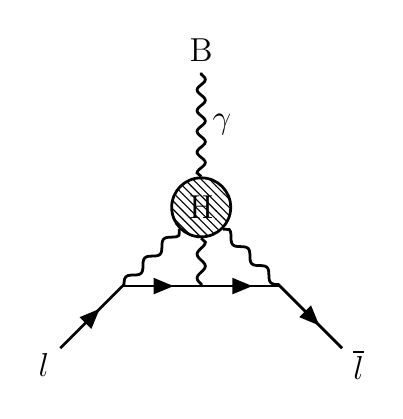
\begin{tikzpicture}[baseline=(o.base)]
		\begin{feynhand}
		\large
		\setlength{\feynhandlinesize}{1pt}
		\vertex [NWblob] (o) at (0,0) {H};
		\vertex (a) at (-2,-2) {$l$}; 
		\vertex (b) at (2,-2) {$\overline l$}; 
		\vertex (c) at (0,2) {B};
		\vertex (d) at (-1,-1);
		\vertex (e) at (1,-1);
		\vertex (f) at (0,-1);
		\propag [fermion] (a) to (d);
		\propag [photon] (d) to (o);
		\propag [anti fermion] (b) to (e);
		\propag [photon] (e) to (o);
		\propag [photon] (c) to [edge label = $\gamma$] (o);
		\propag [fermion] (d) to (f);
		\propag [fermion] (f) to (e);
		\propag [photon] (f) to (o);
		\end{feynhand}
		\end{tikzpicture}
	\caption{H stands for hadrons here...}
	\end{subfigure}
	\hspace{3mm}
	\begin{subfigure}[t]{0.4\textwidth}
	\centering
		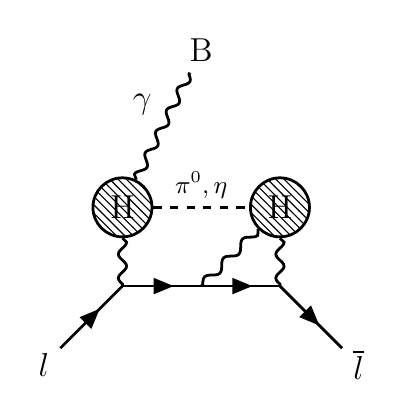
\begin{tikzpicture}[baseline=(o.base)]
		\begin{feynhand}
		\large
		\setlength{\feynhandlinesize}{1pt}
		\vertex [NWblob] (o) at (-1,0) {H};
		\vertex (a) at (-2,-2) {$l$}; 
		\vertex (b) at (2,-2) {$\overline l$}; 
		\vertex (c) at (0,2) {B};
		\vertex (d) at (-1,-1);
		\vertex (e) at (1,-1);
		\vertex (f) at (0,-1);
		\vertex [NWblob] (g) at (1,0) {H};
		\propag [fermion] (a) to (d);
		\propag [photon] (d) to (o);
		\propag [anti fermion] (b) to (e);
		\propag [photon] (e) to (g);
		\propag [photon] (c) to [edge label' = $\gamma$] (o);
		\propag [fermion] (d) to (f);
		\propag [fermion] (f) to (e);
		\propag [photon] (f) to (g);
		\small
		\propag [scalar] (o) to [edge label = {$\pi^{0}, \eta$}] (g);
		\end{feynhand}
		\end{tikzpicture}
	\caption{test2}
	\end{subfigure}
\caption[testfeynmanpicture2]{Feynman diagrams made with \cite{tikz-feynman,tikz-feynhand}.}	
\label{fig:feyn4}
\end{figure}



\subsection{BSM}
\label{subsec:BSM}




-why the muon mdm is important to measure

-talk about chiral flipping stuff




\section{Background / experiment history / new experiment}
\label{sec:Background}




It has the goal of measuring the magnetic moment of the muon, proportional to the $g$ in \gmtwo, to high precision in order to compare to SM theoretical predictions. Because the magnetic moment of particles couple to all existing particles, known or unknown, (source this? reference to a later section?) this provides an avenue through which theories might be constrained, and new physics narrowed down. Indeed this experiment is the latest in a line of such experiments which have measured the magnetic moment of the muon over the past several decades, the last of which measured the magnetic moment of the muon to .54 parts per million (ppm) at Brookhaven National Laboratory (BNL) in 2001 \cite{E821FinalReport}.




The previous \gmtwo experiment at BNL measured a discepancy in the magnetic moment of the muon between theory and experiment with a 2.2 - 2.7 standard deviation. (Cite the final report again?) That disagreement has since grown above 3$\sigma$ \cite{Keshavarzi:2018mgv}, depending on the theoretical analysis approaches used.









\begin{figure}[]
	\centering
	\includegraphics[width=0.9\textwidth]{AlexKPaperComparison}
	\caption[AlexKPaperComparison]{any figures that are directly lifted from someone else's work needs to be cited evertime they're used I believe, even if I cite that work in the text somewhere - \cite{Keshavarzi:2018mgv} }
	\label{fig:AlexKPaperComparison}
\end{figure}




\cleardoublepage

\thispagestyle{myheadings} % should I be including this at the top of every section page??

\graphicspath{ {Body/Figures/ExperimentalOverview/Decay/} {Body/Figures/TrackingFigures/TrackerPics/} {Body/Figures/ExperimentalOverview/Ring/} }

\chapter{Muon g-2 at Fermilab, E989}
\label{chapter:Muon g-2 at Fermilab, E989}

\section{Principle Technique}
\label{sec:PrincipleTechnique}

In a dipole magnetic field, particles will orbit at the cyclotron frequency 
        \begin{align} \label{eq:wc}
        	\omega_{c} = -\frac{Qe}{\gamma m}B,
        \end{align}
and their spins will turn at the precession frequency
        \begin{align} \label{eq:ws}
        	\omega_{s} = -g\frac{Qe}{2m}B - (1-\gamma)\frac{Qe}{\gamma m}B,
        \end{align}
where $Q = \pm 1$ and $e > 0$. The difference between these two frequencies gives
        \begin{align} \label{eq:wasimple}
        	\omega_{a} = \omega_{s} - \omega_{c} = -\frac{g-2}{2}\frac{Qe}{m}B = - a \frac{Qe}{m}B,
        \end{align}
a measureable frequency that is directly proportional to the property of significance, the anamoly a. By measuring the spin difference frequency for muons and the magnetic field B, \amu can be determined. In the presence of an electric field, which is useful in storing the muon beam within a dipole magnetic field, this expands to 
        \begin{align} \label{eq:waelectric}
            \vec{\omega}_{a} = -\frac{Qe}{m} [a_{\mu}\vec{B} - (a_{\mu} - \frac{1}{\gamma^{2}-1})(\vec{\beta} \times \vec{E}) ],
        \end{align}
where now the measurable quanties are vector quantities. Finally, for realistic cases of muon momentum which is non-orthogonal to the magnetic field, the spin difference frequency becomes
        \begin{align} \label{eq:wafinal}
            \vec{\omega}_{a} = -\frac{Qe}{m} [a_{\mu}\vec{B} - a_{\mu} (\frac{\gamma}{\gamma+1})(\vec{\beta} \cdot \vec{B})\vec{B} - (a_{\mu} - \frac{1}{\gamma^{2}-1})(\vec{\beta} \times \vec{E}) ].
        \end{align}
If the motion of the muons is largely perpendicular to the magnetic field, then the second term is small and can be corrected for. If the particles have a momentum of approximately 3.09 GeV/c, the so called ``magic momentum,'' then the third term is small and can be corrected for. These will be talked about later.

In order to measure the spin difference frequency of the muon, a clever technique is used. Decay muons in the pion rest frame are 100\% polarized due to conservation of angular momentum and the fact that the decay neutrino must have a specific helicity. Within a pion beam then the highest and lowest energy decay muons are polarized. Muons will 
decay to positrons with a lifetime of about 2.2 $\mu$s, and the positrons with the highest energies will be correlated with the muon spin, a so called ``self-analyzing'' decay. The single available decay state for a maximum energy positron illustrates this in Figure \ref{fig:MuonDecay}. Thus, by aquiring a large sample of polarized muons and injecting them into a storage ring 

\begin{figure}[]
    \label{fig:MuonDecay}
	\centering
	\includegraphics[width=0.9\textwidth]{MuonDecay}
    \caption[Muon Decay - Max Energy Positron]{Make a new version of this picture, and improve this caption.: The single available decay state for maximum energy decay positrons. Due to the conservation of angular momentum and the single possible helicity states of the decay neutrino and anti-neutrino, the spin of the decay positron is exactly equal to the spin of the muon at the time of the decay.}
\end{figure}



-explain the physics
-explain how we get at the physics with our ring and detectors
-parity violation
-actually write out the decay states before explaining some things - well shouldn't these have been talked about before?? maybe not
-decay probabilities and all that
-don't measure all decay positrons
-By injecting a large ensemble of muons and 
-by measuring a subset of ensemble of muons....
-Careful with spin vs polarization





\begin{figure}[]
    \label{fig:ring}
    \centering
    \includegraphics[width=0.9\textwidth]{ring}
    \caption[ring]{clean up and possibly replace}   
\end{figure}


\section{Accelerator}
\label{sec:Accelerator}


\cite{Stratakis:2017uci}


\section{Detector Systems}
\label{sec:DetectorSystems}

\begin{figure}[]
    \label{fig:TrackerCaloWithLines}
    \centering
    \includegraphics[width=0.9\textwidth]{TrackerCaloWithLines}
    \caption[TrackerCaloWithLines]{clean up and possibly replace}   
\end{figure}


\subsection{Calorimeters}
\label{sec:Calorimeters}

% what they do
% what they are
% how they work


Electromagnetic calorimeters measure the times and energies of decay positrons as they curl inward from the storage region. There are 24 calorimeters located symmetrically around the inside of the ring in close proximity to the vacuum chamber, as shown in Figure \ref{fig:}. They lie close to the storage region in order to measure a large fraction of the total number of observable decay positrons, including the high energy decay positrons which curl inward only slightly more than the muons themselves do. Because they are in close proximity to the storage region and by extension the magnetic field, the calorimeters must be non-magnetic in order to avoid perturbing the magnetic field. Each calorimeter consists of 54 channels of PbF\textsubscript{2} crystals arrayed in a 6 high by 9 wide array, which measure Cerenkov light emitted by the impinging positrons as they pass through the crystals \cite{Fienberg:2014kka}. (Picture of single calo and its crystals here.) Each crystal is 2.5 x 2.5 x 14 cm\textsuperscript{3}. The light is read out by large area silicon photo-multiplier (SiPM) sensors.


In order to determine \amu to the precision goal, there are modest requirements on the performance of the calorimeters. They must have a relative energy resolution of better than 5\% at 2 GeV, in order for proper event selection \cite{TDR}. They must have a timing resolution of better than 100 ps. The calorimeters must be able to resolve multiple incoming hits through temporal or spatial separation at 100\% efficiency for time separations of greater than 5 ns in order to reduce the pileup systematic error due to the high rate. Finally, the gain of the measured hits must be stable to $<$ 0.1\% over a 200 $\mu$s time period within a fill, and unaffected by a pulse arriving in the same channel a few nanoseconds earlier. The long term gain stability over a time period of order seconds must be $<$ 1\%.

(I've condensed quite a bit this section from the TDR - is that okay?)


To satisy these requirements SiPM sensors were chosen over PMTS...



and is wrapped in black Tedlar\textregistered\ foil



\cite{Kaspar:2016ofv} % second calo paper I need to cite



\subsection{Laser System}
\label{LaserSystem}
% should make this it's own section

For the gain, there is a laser system...

% make sure these are ordered properly
\cite{Anastasi:2015ssy}
\cite{Anastasi:2016luh}
\cite{Anastasi:2017sos}



% magnetic nature of calorimeters

% energy resolution
% gain
% high rate
% acceptance

% design of the vacuum chambers in order to...

% picture of calo placement
% picture of actual calo station




\subsection{Template Fitting}
\label{sec:TemplateFitting}





\subsection{Straw Trackers}
\label{sec:StrawTrackers}

The Muon \gmtwo Experiment at Fermilab uses straw tracking detectors to measure decay positron trajectories for the purpose of determining the muon beam distribution and its characteristics (and other things....). By fitting these tracks and extrapolating back to the average decay point, the beam can be characterized in a non-destructive fashion. See section blah. This is important because of the need for matching the average observed magnetic field of the decaying muons and their resulting decay positron directions which result in the \wa frequency.

The trackers are also useful for determining general beam diagnostics as well as the pitch correction and to a lesser extent the electric field correction (careful here). Cross-checking separately for pileup removal, hit verification, etc. is a powerful tool. Combining them in order to provide the muon distribution that the calorimeters directly see for the \wa calculation is perhaps the most important role of the tracker. With three trackers, approximately 5\% of decaying muons will result in measureable positron tracks assuming no pileup in the tracker, many of which do not hit the nearest calorimeter.

Each tracker module consists of 4 layers of 32 straws with a stereo angle of 7.5 degrees, the first two ``U'' layers oriented with the tops of the straws at a greater radial position, and the second two ``V'' layers oriented with the bottoms of the straws at a greater radial position. A tracking module is shown in Figure \ref{fig:tracker}. There are 2 tracker stations located in front of calorimeters 13 and 19, or at approximately 180 and 270 degrees counting clockwise from the top most point of the ring where the inflector resides. Figure \ref{fig:WorldCoordSys} shows this. (A third station sits empty after the inflector.) Each station consists of 8 tracking modules arranged in a staircase pattern that follows the curvature of the ring as seen in Figure \ref{fig:staircase}.

\begin{figure}[]
    \label{fig:tracker}
    \centering
    \includegraphics[width=0.9\textwidth]{Tracker}
    \caption[Tracker module]{Shown is a picture of one of the many tracking modules used in the Muon \gmtwo experiment. The first layer of straws with a stereo angle of 7.5 degrees can be seen, with the other 3 straw layers hiding behind it. The beam direction is roughly into the page in this picture, to the left of the end of the module, and this view is what the decay positrons will see.}
\end{figure}

\begin{figure}[]
    \label{fig:staircase}
    \centering
    \includegraphics[width=0.9\textwidth]{trackerStation}
    \caption[Tracker module arrangement]{Tracker modules are arranged in the shown staircase pattern. In green and dark blue is the edge of the vacuum chamber (where the dark blue identifies the modification that was made to the old vacuum chambers), and it can be seen that vacuum chamber walls lie at the ends of the outside tracking modules. The position of a calorimeter can be seen in cyan at the right. The dark red spots are the locations of the outside magnet pole tips. From the shown geometry one can see that many positrons will hit either the tracker or the calorimeter but not both due to the acceptance differences.}
\end{figure}

In order to reduce the amount of multiple scattering within the straw tracking chambers as particles pass through them, the material of the straw trackers is minimized. Each straw is made of mylar foil, within which a 25 $\mu$m radius tungsten wire resides, and is filled with Argon-Ethane gas \cite{something}. Fast moving particles ionize the gas as they pass through it, and the resulting ions are drawn to the wire which is held at high voltage. When they reach the wire (and the mylar) a signal can be read out which tells us that a particle was seen to pass through the straw. By combining many such signals in a brief time span, we are able to construct tracks of incidient particles. (See section blah.) The resolution of hits within the straws is approximately 150 $\mu$m \cite{something}.

The signals of the straws are read out through...



\cleardoublepage

%!TEX root = ../thesis.tex

\thispagestyle{myheadings}

\chapter{Magnetic Field Measurement}
\label{chapter:MagneticFieldMeasurement}

\section{Trolley}
\label{sec:Trolley}

\section{Opera Simulations}
\label{sec:OperaSimulations}

Where does this section really go?

\cleardoublepage

\chapter{Straw Tracking}
\label{chapter:Straw Tracking}
\thispagestyle{myheadings} % should I be including this at the top of every section page??


\graphicspath{ {Body/Figures/TrackingFigures/} {Body/Figures/TrackingFigures/MainPlots/} {Body/Figures/TrackingFigures/MainPlots/PlanePlots/} {Body/Figures/TrackingFigures/MainPlots/PullPlots/} {Body/Figures/TrackingFigures/MainPlots/Residuals/} {Body/Figures/TrackingFigures/eLoss/} {Body/Figures/TrackingFigures/CoordSys/} {Body/Figures/TrackingFigures/TrackerPics/} {Body/Figures/TrackingFigures/Field/} {Body/Figures/TrackingFigures/TrackingFlow/} {Body/Figures/TrackingFigures/LeftRight/} {Body/Figures/TrackingFigures/Misc/}}

\section{Straw Tracking Intro}
\label{sec:StrawTrackingIntro}


  The Muon \gmtwo Experiment at Fermilab uses straw tracking detectors to measure decay positron trajectories for the purpose of determining the muon beam distribution and its characteristics. By fitting these tracks and extrapolating back to the average decay point, the beam can be characterized in a non-destructive fashion. This is important because of the need for matching the average observed magnetic field of the decaying muons and their resulting decay positron directions which result in the \wa frequency, as seen in
        \begin{align} \label{eq:wa}
            \vec{\omega}_{a} = \frac{e}{m} [a_{\mu}\vec{B} - a_{\mu} (\frac{\gamma}{\gamma+1})(\vec{\beta} \cdot \vec{B})\vec{B} - (a_{\mu} - \frac{1}{\gamma^{2}-1})(\vec{\beta} \times \vec{E}) ].
        \end{align}
  The trackers are also useful for determining general beam diagnostics as well as the pitch correction and to a lesser extent the electric field correction, terms 2 and 3 in Equation \ref{eq:wa} respectively. The tracking analysis can be done independently of, or in tandem with, the calorimeters. Cross-checking separately for pileup removal, hit verification, etc. is a powerful tool. Combining them in order to provide the muon distribution that the calorimeters directly see for the \wa calculation is perhaps the most important role of the tracker. (An EDM analysis needs to be done separately.) It is worth noting that there is a large percentage of tracks hitting the calorimeters that hit zero or only a small number of tracking modules, which this Geane fitting code is not capable of handling. With three trackers, approximately 5\% of decaying muons will result in measureable positron tracks assuming no pileup in the tracker, many of which do not hit the nearest calorimeter. Note that the integration of the two detector systems in the code (tracker-calo matching) has just recently been initiated, \href{https://gm2-docdb.fnal.gov/cgi-bin/private/ShowDocument?docid=7514}{DocDB 7514}.

  Each tracker module consists of 4 layers of 32 straws with a stereo angle of 7.5 degrees, the first two ``U'' layers oriented with the tops of the straws at a greater radial position, and the second two ``V'' layers oriented with the bottoms of the straws at a greater radial position. A tracking module is shown in Figure \ref{fig:tracker}. There are 3 tracker stations located at the 0th, 12th, and 18th sections of the ring, counting clockwise from the top most point of the ring where the inflector resides. Figure \ref{fig:WorldCoordSys} shows this. (Station 18 was installed for the commissioning run, with station 0 planned for the fall. Station 12 might or might not be installed sometime in the future.) Each station consists of 8 tracking modules arranged in a staircase pattern that follows the curvature of the ring as seen in Figure \ref{fig:staircase}. Further hardware and electronics information regarding the trackers will be omitted in this document.

\begin{figure}[]
\caption[Tracker module]{Shown is a picture of one of the many tracking modules used in the Muon \gmtwo experiment. The first layer of straws with a stereo angle of 7.5 degrees can be seen, with the other 3 straw layers hiding behind it. The beam direction is roughly into the page in this picture, to the left of the end of the module, and this view is what the decay positrons will see.}
\centering
\includegraphics[width=0.9\textwidth]{Tracker}
\label{fig:tracker}
\end{figure}

\begin{figure}[]
\caption[Tracker module arrangement]{Tracker modules are arranged in the shown staircase pattern. In green and dark blue is the edge of the vacuum chamber (where the dark blue identifies the modification that was made to the old vacuum chambers), and it can be seen that vacuum chamber walls lie at the ends of the outside tracking modules. The position of a calorimeter can be seen in cyan at the right. The dark red spots are the locations of the outside magnet pole tips. From the shown geometry one can see that many positrons will hit either the tracker or the calorimeter but not both due to the acceptance differences.}
\centering
\includegraphics[width=0.9\textwidth]{trackerStation}
\label{fig:staircase}
\end{figure}


  Because of the proximity of the trackers to the muon beam, they will lie within a region of varying magnetic field. The radial field of the trackers rises from 0 Tesla at the outer ends to roughly .3 Tesla at the inner top and bottom ends, and the vertical field drops approximately 50\% from the storage dipole field of 1.451 Tesla. Shown in Figures \ref{fig:operaBy} and \ref{fig:operaBx} is the location of the tracker with respect to the horizontal and vertical fields respectively. These large field gradients over the tracking detector region and the long extrapolation distance back to the muon decay point are special to Muon \gmtwo. This is one of the main motivations for using the Geane (Geometry and Error Propagation) fitting algorithm and routines, which has direct access to the field.

\begin{figure}[]
\caption[Vertical magnetic field from Opera2D]{Shown is the vertical field of the \gmtwo magnet in and around the storage region as calculated in Opera 2D. The center of the storage region lies at 7.112 m along the x axis. The black box shows the rough location of the tracker with respect to the field (size exaggerated slightly). It can be seen that there is a large inhomogeneity within the tracker space, goring from left to right.}
\centering
\includegraphics[width=0.9\textwidth]{operaBy}
\label{fig:operaBy}
\end{figure}

\begin{figure}[]
\caption[Horizontal magnetic field from Opera2D]{Shown is the radial field of the \gmtwo magnet in and around the storage region as calculated in Opera 2D. The center of the storage region lies at 7.112 m along the x axis. The black box shows the rough location of the tracker with respect to the field (size exaggerated slightly). It can be seen that there is a large homogeneity at the inner upper and lower ends compared to the right center. The shape of the pole pieces and tips can readily be seen.}
\centering
\includegraphics[width=0.9\textwidth]{operaBx}
\label{fig:operaBx}
\end{figure}

  The Geane fitting routines originated in Fortran with the EMC collaboration, and was used in the precursor E821 experiment as well as the PANDA experiment with some success \cite{geanemanual}, \cite{Lavezzi}. (I'm not actually aware of a useful reference for it's use in E821, and there are some other instances of its use as well in other experiments. In E821 there was a single tracking chamber which was never put to full use.) The core error propagation routines were at some point added to Geant4 under the error\_propagation directory which is included in all default installs. The tracking code strengths lie with its direct implementation and access to the Geant4 geometry and field, and its ability to handle the field inhomogeneties. The Geane fitting algorithm code which makes use of the Geant4 error propagation routines follows the structure of \cite{geanemanual} and is detailed in the \hyperref[sec:Formalism]{Formalism} section in this paper. It is a relatively straight forward least squares global \chisq minimization algorithm. 








\section{Track Finding}
\label{sec:Track Finding}

\section{Track Fitting}
\label{sec:Track Fitting}

\section{Track Extrapolation}
\label{sec:Track Extrapolation}

\cleardoublepage

%!TEX root = ../thesis.tex

\chapter{\texorpdfstring{\wa}{wa} Measurement}
\label{chapter:SpinPrecessionMeasurement}
\thispagestyle{myheadings}

\section{Details of Run 1}
\label{sec:Data}

\section{Reconstruction}
\label{sec:ReconWest}

\cite{AFThesis}

\subsection{Clustering}
\label{sec:Clustering}

\section{Histogramming}
\label{sec:Histogramming}

\section{Fitting}
\label{sec:Fitting}

\section{Systematic Errors}
\label{sec:Systematic Errors}



\cleardoublepage

\cleardoublepage

%!TEX root = ../thesis.tex

\thispagestyle{myheadings} % should I be including this at the top of every section page??

\chapter{Conclusion}
\label{chapter:Conclusion}


The final results for the blinded \R values for the Run~1 precession frequency analysis datasets along with their total statistical and systematic errors is given in \tabref{tab:FinalResults}.


\begin{table}[]
\centering
% \small
% \setlength\tabcolsep{10pt}
\renewcommand{\arraystretch}{1.2}
\begin{tabular*}{\linewidth}{@{\extracolsep{\fill}}lcccc}
  \hline
    \multicolumn{5}{c}{\textbf{Run~1 Final Results}} \\
  \hline\hline
    Dataset & \multicolumn{1}{c}{Mean \R} & \multicolumn{1}{c}{$\sigma_{\text{stat.}}$} & \multicolumn{1}{c}{$\sigma_{\text{sys.}}$} & \multicolumn{1}{c}{$\sigma_{\text{tot.}}$} \\ 
  \hline
  	60h & -20.5562 & 1.3581 & 0.1441 & 1.3657 \\
  	HighKick & -17.4755 & 1.4112 & 0.1995 & 1.4252 \\
  	9d & -17.7182 & 0.9033 & 0.1945 & 0.9240 \\
  	Endgame & -17.3406 & 0.6393 & 0.2042 & 0.6711 \\
  \hline
  Total & & 0.4605 & & 0.4757 \\
  \hline
\end{tabular*}
\caption[]{Units are in ppm.}
\label{tab:FinalResults}
\end{table}







-quote the mean R values for the different datasets along with the systematic and statistical errors

-calculate what the final weighted statistical error will be approximately

-mention further ongoing dqc work to clean up the datasets before publication
-mention the datasets are not quite final - mention lowkick

-give preliminary values for the e field and pitch correction numbers


-should maybe do what aaron did and give a number for the expected magnetic field error and then the error on a mu

-have a table with the statistical and systematic errors side by side - or a table with the results




\cleardoublepage

%%%%%%%%%%%%%%%%%%%%%%%%%%%%%%%%%%%%%%%%%

%\ The appendix
\begin{appendices}
\include{Appendix/Appendix}
\end{appendices}

%==========================================================================%
% Bibliography
\newpage
\singlespace
\printbibliography
\cleardoublepage

%==========================================================================%
% Curriculum Vitae
%!TEX root = ../thesis.tex

% \addcontentsline{toc}{chapter}{Curriculum Vitae}

\thispagestyle{myheadings}

% \chapter*{test}
% \addcontentsline{toc}{chapter}{Curriculum Vitae}


% original template from https://www.overleaf.com/latex/templates/simple-resume/gtrrjrsrfkvk


% \usepackage{latexsym}
% \usepackage[empty]{fullpage}
% \usepackage{titlesec}
% \usepackage{marvosym}
% \usepackage[usenames,dvipsnames]{color}
% \usepackage{verbatim}
% \usepackage{enumitem}
% \usepackage[pdftex, hidelinks]{hyperref}
% \usepackage{fancyhdr}

% \usepackage[charter]{mathdesign} % Bitstream Charter
% \usepackage{newpxtext,newpxmath} % Palatino


%-------------------------
% Custom commands
\newcommand{\resumeItem}[2]{
  \item\small{
    \textbf{#1}{: #2 \vspace{-2pt}}
  }
}

\newcommand{\resumeItemNoBullet}[2]{
  \item[]\small{
    \hspace{-9pt}\textbf{#1}{: #2 \vspace{-6pt}}
  }
}

\newcommand{\resumeSubheading}[4]{
  \vspace{-1pt}\item[]
  \begin{tabular*}{0.98\textwidth}{l@{\extracolsep{\fill}}r}
      \hspace{-10pt}\textbf{#1} & #2 \\
      \hspace{-10pt}\textit{\small#3} & \textit{\small #4} \\
    \end{tabular*}\vspace{-5pt}
}

\newcommand{\resumeSubItem}[2]{\resumeItem{#1}{#2}\vspace{-4pt}}

\renewcommand{\labelitemii}{$\circ$}

\newcommand{\resumeSubHeadingListStart}{\begin{itemize}[leftmargin=*]}
\newcommand{\resumeSubHeadingListEnd}{\end{itemize}}
\newcommand{\resumeItemListStart}{\begin{itemize}}
\newcommand{\resumeItemListEnd}{\end{itemize}\vspace{-5pt}}

% custom commands
\newcommand{\shorterSection}[1]{\vspace{-10pt}\section{#1}}

%-------------------------------------------
%%%%%%  CV STARTS HERE  %%%%%%%%%%%%%%%%%%%%%%%%%%%%


%----------HEADING-----------------
\begin{center}
  \textbf{{\huge Nicholas Kinnaird}} \\
  \small 512-922-0534 $\vert$ nickkinn@bu.edu $\vert$ 1101 Iroquois Ave Apt 1401, Naperville, IL 60563
\end{center}

%-----------EDUCATION-----------------
\shorterSection{Education}
  \resumeSubHeadingListStart
    \resumeSubheading
      {Boston University}{Boston, MA}
      {Ph.D. in Physics}{2020}{
      \resumeItemNoBullet{Dissertation}{Muon Spin Precession Frequency Extraction and Decay Positron Track Fitting in Run 1 of the Fermilab Muon \gmtwo Experiment}
      % \resumeItemNoBullet{Relevant Coursework}{Advanced Machine Learning, Advanced Database Management Systems, Applied Artificial Intelligence, AI: Innovation \& Entrepreneurship, Data Mining \& Text Mining, Introduction to Data Science}
    }
    \resumeSubheading
      {Boston University}{Boston, MA}
      {M.A. in Physics}{2016}{
      % \resumeItemNoBullet{Relevant Coursework}{Advanced Machine Learning, Advanced Database Management Systems, Applied Artificial Intelligence, AI: Innovation \& Entrepreneurship, Data Mining \& Text Mining, Introduction to Data Science}
    }
    \resumeSubheading
      {University of Texas at Austin}{Austin, TX}
      {B.S. in Physics}{2013}
      % \resumeItemNoBullet{Relevant Coursework}{Analysis \& Design of Algorithms, Data Structures using C, Operating Systems, Pattern Recognition}
    \resumeSubheading
      {University of Texas at Austin}{Austin, TX}
      {B.S. in Mathematics}{2013}{}
  \resumeSubHeadingListEnd

% %-----------SKILLS-----------------
% \shorterSection{Skills}
%   \resumeSubHeadingListStart
%   \small
%     \item{
%      \textbf{Languages}{: Python, C++, SQL, Java, Swift}
%      \hfill
%      \textbf{Technologies}{: GCP, AWS, GitHub, GitLab, Docker}
%     }
%     \vspace{-5pt}
%     \item{
%      \textbf{Libraries}{: TensorFlow, PyTorch, Keras, Scikit-Learn, Numpy, Pandas, Spark, Jupyter, OpenCV, PIL, OpenCL, OpenGL, CUDA}
%     }
% \resumeSubHeadingListEnd

% %-----------EXPERIENCE-----------------
% \shorterSection{Experience}
%   \resumeSubHeadingListStart

%     \resumeSubheading
%       {CCC Information Services}{Chicago, IL}
%       {R\&D Engineer Intern (Machine Learning)}{May 2018 - Present}
%       \resumeItemListStart
%         \resumeItem{RotNet}
%           {Designed and trained a shallow CNN to classify rotated images. Achieved F1-score of 0.99 on test set of 1M+ images}
%         \resumeItem{TagNet}
%           {A computer vision model to classify views of automobile images
%             \begin{itemize}
%                 \item Implemented an expectation maximization algorithm to sample and classify images from 6M+ unlabeled images to prepare a clean dataset of 100K+ images for training
%                 \item Designed and trained a low-complexity CNN to classify 20+ views of automobile images resulting in 30\% improvement in  F1-score compared to SVM model
%                 \item Reduced model complexity and size by 40\% by freezing model and performing post-training quantization
%             \end{itemize}
%           }
%         \resumeItem{TVR}
%           {A computer vision model to determine if image is total loss or repairable
%           \begin{itemize}
%               \item Trained ensemble of CNN architectures on 1M+ automobile images to classify vehicles as total loss or repairable resulting in 25\% higher weighted F1-score and 60\% decrease in model size compared to older iteration
%               \item Incorporated first notice of loss information using NLP to increase  F1-score by 10\%
%           \end{itemize}
%           }
%       \resumeItemListEnd

%     \resumeSubheading
%       {Reliance Communications}{Mumbai, India}
%       {Software Engineer Intern}{May 2016 - Aug 2016}
%       \resumeItemListStart
%         \resumeItem{Optimal Node Search}
%           {Implemented Dijkstra's algorithm on 10K+ network nodes to find shortest path for signal propagation resulting in 25\% reduction in costs}
%       \resumeItemListEnd

%     \resumeSubheading
%       {OSSCube}{New Delhi, India}
%       {Software Engineer Intern}{May 2015 - Aug 2015}
%       \resumeItemListStart
%         \resumeItem{Squeek Twitter iOS}
%           {Designed and developed Twitter client using Fabric SDK}
%       \resumeItemListEnd

%   \resumeSubHeadingListEnd

% %-----------PROJECTS-----------------
% \shorterSection{Projects}
%   \resumeSubHeadingListStart
%     \resumeSubItem{OCR using Conditional Random Fields}
%      {A probabilistic graphical model for sequential character recognition
%         \vspace{-5pt}
%         \begin{itemize}
%             \item Implemented a CRF in $O(m|\mathcal{Y}|^2)$ time to achieve a 84\% letter-wise accuracy on UPenn OCR dataset
%             \item Implemented OpenMPI CRF using PETSc and Tao to achieve 77.1\% letter-wise accuracy
%         \end{itemize}
%      }
%     \resumeSubItem{ARYouThereYet}{An augmented reality application developed on ARKit with dynamic AR nodes}
%     \resumeSubItem{Aspect-based Sentiment Analysis}
%       {Implemented Deep Memory Networks to achieve 78.66\% accuracy, 0.69 F1-score on SemEval 2014 dataset}
%     \resumeSubItem{Iris Speech to Code}
%       {A natural speech to code converter for aiding programmers with disabilities
%         \vspace{-5pt}
%         \begin{itemize}
%             \item Trained an intent classification model in Microsoft Luis to classify 15+ classes or commands
%             \item Implemented a message passing protocol using RabbitMQ to broker messages between Google API, ElectronJS, and VS Code
%         \end{itemize}
%       }
%     \resumeSubItem{AI Lifeguard}{Trained a 3D-CNN model on Microsoft Azure for action localization on drowning people in swimming pools. Achieved mean IOU score of 0.45}
%   \resumeSubHeadingListEnd

% %-----------Addtional Experience & Achievements-----------------
% \shorterSection{Additional Experience \& Achievements}
%   \resumeSubHeadingListStart
%   \small
%     \item{Presented poster on \textit{Tiramisu DenseNet Architecture for Precise Segmentation} for Intel AI at \textbf{CVPR 2018}}
%     \vspace{-5pt}
%     \item{Selected as an \textbf{Intel AI Student Ambassador} (only 150 students) to research, publish, and share work on machine learning and deep learning}
%     \vspace{-5pt}
%     \item{Won \textit{Best Microsoft Hack} out of 220 teams at \textbf{HackHarvard 2017}}
%     \vspace{-5pt}
%     \item{Placed 16/50 at Google Games: Campus Edition 2017 at UIC}
%     \vspace{-5pt}
%     \item{Won \textit{Best Technical Innovation} award (out of 800 students) at \textbf{Amity University Convocation 2017}}
%     \vspace{-5pt}
%     \item{Elected as a \textit{Vice-Chair} for \textbf{ACM Amity Student Chapter} out of 800 students at Amity University based on high-achieving and technically strong undergraduate students}
%   \resumeSubHeadingListEnd
%-------------------------------------------
\end{document}


%==========================================================================%
\end{document}
